\documentclass[
  shownotes,
  xcolor={svgnames},
  hyperref={colorlinks,citecolor=DarkBlue,linkcolor=DarkRed,urlcolor=DarkBlue}
  , aspectratio=169]{beamer}
\usepackage{animate}
\usepackage{amsmath}
\usepackage{amsfonts}
\usepackage{amssymb}
\usepackage{pifont}
\usepackage{mathpazo}
%\usepackage{xcolor}
\usepackage{multimedia}
\usepackage{fancybox}
\usepackage[para]{threeparttable}
\usepackage{multirow}
\setcounter{MaxMatrixCols}{30}
\usepackage{subcaption}
\usepackage{graphicx}
\usepackage{lscape}
\usepackage[compatibility=false,font=small]{caption}
\usepackage{booktabs}
\usepackage{ragged2e}
\usepackage{chronosys}
\usepackage{appendixnumberbeamer}
\usepackage{animate}
\setbeamertemplate{caption}[numbered]
\usepackage{color}
%\usepackage{times}
\usepackage{tikz}
\usepackage{comment} %to comment
%% BibTeX settings
\usepackage{natbib}
\bibliographystyle{apalike}
\bibpunct{(}{)}{,}{a}{,}{,}
\setbeamertemplate{bibliography item}{[\theenumiv]}

% Defines columns for bespoke tables
\usepackage{array}
\newcolumntype{L}[1]{>{\raggedright\let\newline\\\arraybackslash\hspace{0pt}}m{#1}}
\newcolumntype{C}[1]{>{\centering\let\newline\\\arraybackslash\hspace{0pt}}m{#1}}
\newcolumntype{R}[1]{>{\raggedleft\let\newline\\\arraybackslash\hspace{0pt}}m{#1}}


\usepackage{xfrac}


\usepackage{multicol}
\setlength{\columnsep}{0.5cm}

% Theme and colors
\usetheme{Boadilla}

% I use steel blue and a custom color palette. This defines it.
\definecolor{andesred}{HTML}{af2433}

% Other options
\providecommand{\U}[1]{\protect\rule{.1in}{.1in}}
\usefonttheme{serif}
\setbeamertemplate{itemize items}[default]
\setbeamertemplate{enumerate items}[square]
\setbeamertemplate{section in toc}[circle]

\makeatletter

\definecolor{mybackground}{HTML}{82CAFA}
\definecolor{myforeground}{HTML}{0000A0}

\setbeamercolor{normal text}{fg=black,bg=white}
\setbeamercolor{alerted text}{fg=red}
\setbeamercolor{example text}{fg=black}

\setbeamercolor{background canvas}{fg=myforeground, bg=white}
\setbeamercolor{background}{fg=myforeground, bg=mybackground}

\setbeamercolor{palette primary}{fg=black, bg=gray!30!white}
\setbeamercolor{palette secondary}{fg=black, bg=gray!20!white}
\setbeamercolor{palette tertiary}{fg=white, bg=andesred}

\setbeamercolor{frametitle}{fg=andesred}
\setbeamercolor{title}{fg=andesred}
\setbeamercolor{block title}{fg=andesred}
\setbeamercolor{itemize item}{fg=andesred}
\setbeamercolor{itemize subitem}{fg=andesred}
\setbeamercolor{itemize subsubitem}{fg=andesred}
\setbeamercolor{enumerate item}{fg=andesred}
\setbeamercolor{item projected}{bg=gray!30!white,fg=andesred}
\setbeamercolor{enumerate subitem}{fg=andesred}
\setbeamercolor{section number projected}{bg=gray!30!white,fg=andesred}
\setbeamercolor{section in toc}{fg=andesred}
\setbeamercolor{caption name}{fg=andesred}
\setbeamercolor{button}{bg=gray!30!white,fg=andesred}


\usepackage{fancyvrb}
\newcommand{\VerbBar}{|}
\newcommand{\VERB}{\Verb[commandchars=\\\{\}]}
\DefineVerbatimEnvironment{Highlighting}{Verbatim}{commandchars=\\\{\}}
% Add ',fontsize=\small' for more characters per line
\usepackage{framed}
\definecolor{shadecolor}{RGB}{248,248,248}
\newenvironment{Shaded}{\begin{snugshade}}{\end{snugshade}}
\newcommand{\AlertTok}[1]{\textcolor[rgb]{0.94,0.16,0.16}{#1}}
\newcommand{\AnnotationTok}[1]{\textcolor[rgb]{0.56,0.35,0.01}{\textbf{\textit{#1}}}}
\newcommand{\AttributeTok}[1]{\textcolor[rgb]{0.77,0.63,0.00}{#1}}
\newcommand{\BaseNTok}[1]{\textcolor[rgb]{0.00,0.00,0.81}{#1}}
\newcommand{\BuiltInTok}[1]{#1}
\newcommand{\CharTok}[1]{\textcolor[rgb]{0.31,0.60,0.02}{#1}}
\newcommand{\CommentTok}[1]{\textcolor[rgb]{0.56,0.35,0.01}{\textit{#1}}}
\newcommand{\CommentVarTok}[1]{\textcolor[rgb]{0.56,0.35,0.01}{\textbf{\textit{#1}}}}
\newcommand{\ConstantTok}[1]{\textcolor[rgb]{0.00,0.00,0.00}{#1}}
\newcommand{\ControlFlowTok}[1]{\textcolor[rgb]{0.13,0.29,0.53}{\textbf{#1}}}
\newcommand{\DataTypeTok}[1]{\textcolor[rgb]{0.13,0.29,0.53}{#1}}
\newcommand{\DecValTok}[1]{\textcolor[rgb]{0.00,0.00,0.81}{#1}}
\newcommand{\DocumentationTok}[1]{\textcolor[rgb]{0.56,0.35,0.01}{\textbf{\textit{#1}}}}
\newcommand{\ErrorTok}[1]{\textcolor[rgb]{0.64,0.00,0.00}{\textbf{#1}}}
\newcommand{\ExtensionTok}[1]{#1}
\newcommand{\FloatTok}[1]{\textcolor[rgb]{0.00,0.00,0.81}{#1}}
\newcommand{\FunctionTok}[1]{\textcolor[rgb]{0.00,0.00,0.00}{#1}}
\newcommand{\ImportTok}[1]{#1}
\newcommand{\InformationTok}[1]{\textcolor[rgb]{0.56,0.35,0.01}{\textbf{\textit{#1}}}}
\newcommand{\KeywordTok}[1]{\textcolor[rgb]{0.13,0.29,0.53}{\textbf{#1}}}
\newcommand{\NormalTok}[1]{#1}
\newcommand{\OperatorTok}[1]{\textcolor[rgb]{0.81,0.36,0.00}{\textbf{#1}}}
\newcommand{\OtherTok}[1]{\textcolor[rgb]{0.56,0.35,0.01}{#1}}
\newcommand{\PreprocessorTok}[1]{\textcolor[rgb]{0.56,0.35,0.01}{\textit{#1}}}
\newcommand{\RegionMarkerTok}[1]{#1}
\newcommand{\SpecialCharTok}[1]{\textcolor[rgb]{0.00,0.00,0.00}{#1}}
\newcommand{\SpecialStringTok}[1]{\textcolor[rgb]{0.31,0.60,0.02}{#1}}
\newcommand{\StringTok}[1]{\textcolor[rgb]{0.31,0.60,0.02}{#1}}
\newcommand{\VariableTok}[1]{\textcolor[rgb]{0.00,0.00,0.00}{#1}}
\newcommand{\VerbatimStringTok}[1]{\textcolor[rgb]{0.31,0.60,0.02}{#1}}
\newcommand{\WarningTok}[1]{\textcolor[rgb]{0.56,0.35,0.01}{\textbf{\textit{#1}}}}
\usepackage{graphicx}
\makeatletter

\definecolor{airforceblue}{rgb}{0.36, 0.54, 0.66}

\usepackage{tikz}
% Tikz settings optimized for causal graphs.
\usetikzlibrary{shapes,decorations,arrows,calc,arrows.meta,fit,positioning}
\tikzset{
    -Latex,auto,node distance =1 cm and 1 cm,semithick,
    state/.style ={ellipse, draw, minimum width = 0.7 cm},
    point/.style = {circle, draw, inner sep=0.04cm,fill,node contents={}},
    bidirected/.style={Latex-Latex,dashed},
    el/.style = {inner sep=2pt, align=left, sloped}
}


\makeatother






%%%%%%%%%%%%%%% BEGINS DOCUMENT %%%%%%%%%%%%%%%%%%

\begin{document}
 
\title[Lecture 18]{Lecture 18: \\ Lasso for Causal Inference}
\subtitle{Big Data and Machine Learning for Applied Economics \\ Econ 4676}
\date{\today}

\author[Sarmiento-Barbieri]{Ignacio Sarmiento-Barbieri}
\institute[Uniandes]{Universidad de los Andes}


\begin{frame}[noframenumbering]
\maketitle
\end{frame}

%%%%%%%%%%%%%%%%%%%%%%%%%%%%%%%%%%%



%----------------------------------------------------------------------% 

\begin{frame}
\frametitle{Agenda}

\tableofcontents

\end{frame}

%----------------------------------------------------------------------%
\section{Recap }


%----------------------------------------------------------------------%
\begin{frame}[fragile]
\frametitle{Recap: Regularization}


\begin{itemize}
\item For $\lambda \geq 0$ given, consider minimizing the following objective function
\item Lasso:
\begin{align}
min_{\beta} L(\beta) = \sum_{i=1}^n (y_i-\beta_0 - \sum_{j=1}^p x_{ij}\beta_j)^2 + \lambda \sum_{j=1}^p |\beta_j| 
\end{align}
\item Ridge:
\begin{align}
min_{\beta} R(\beta) = \sum_{i=1}^n (y_i-\beta_0 - \sum_{j=1}^p x_{ij}\beta_j)^2 + \lambda \sum_{j=1}^p (\beta_j)^2
\end{align}
\end{itemize}

\end{frame}


%----------------------------------------------------------------------%
\begin{frame}[fragile]
\frametitle{Recap: Regularization}

\begin{itemize}
\item Elastic net: happy medium. 
  \begin{itemize}
    \item Good job at prediction and selecting variables
  \end{itemize}
\end{itemize}

\begin{align}
min_{\beta} NEL(\beta) &= \sum_{i=1}^n (y_i-\beta_0 - \sum_{j=1}^p x_{ij}\beta_j)^2 + \lambda \sum_{j=1}^p (\beta_j)^2 + \lambda \sum_{j=1}^p |\beta_j| 
\end{align}


\begin{itemize}
 \item Mixes Ridge and Lasso
 \item Lasso selects predictors
 \item Strict convexity part  of the penalty (ridge) solves the grouping instability problem 
 \scriptsize
 \item H.W.: $\beta_{OLS}>0$ one predictor standarized
 \begin{align}
\hat{\beta}_{naive\,EN}= \frac{\left(\hat{\beta}_{OLS}-\frac{\lambda_1}{2}\right)_{+}}{1+\lambda_2}
\end{align}
\end{itemize}

%The second term encourages highly correlated features to be averaged, while the first term encourages a sparse solution in the coefficients of these averaged features. The elastic net penalty can be used with any linear model, in particular for regression or classification. pg 662 Elements
\end{frame}

%----------------------------------------------------------------------%
\begin{frame}[fragile]
\frametitle{Elastic Net}

\begin{itemize}
\item Elastic Net: reescaled version of Naive version
\item Double Shrinkage introduces ``too'' much bias, {\it final} version ``corrects'' for this
\end{itemize}
\bigskip
\begin{align}
\hat{\beta}_{EN}= \frac{1}{\sqrt{1+\lambda_2}}\hat{\beta}_{naive\,EN}
\end{align}
\bigskip
\begin{itemize}
  \item Careful sometimes software asks.
  \item How to choose $(\lambda_1,\lambda_2)$? $\rightarrow$ Bidimensional Crossvalidation
  \item Zou, H. \& Hastie, T. (2005)
\end{itemize}

\end{frame}

%----------------------------------------------------------------------%
\section{Lasso for Causality}
%----------------------------------------------------------------------%
\begin{frame}[fragile]
\frametitle{Model Selection When the Goal is Causal Inference}
\framesubtitle{Motivation}


\begin{itemize}
\item In this course our objective is prediction
\medskip
\pause
\item But since we are economists, inference is always there
\pause
\medskip
\item Can we use some of these models to do causal inference?
\medskip

\item We are going to see how we can use lasso when inference is the main goal
\end{itemize}

\end{frame}
%----------------------------------------------------------------------%
\begin{frame}[fragile]
\frametitle{Model Selection When the Goal is Causal Inference}

Let's start with the following model
\medskip
\begin{align}
  y_i = \alpha D_i + g(X_i) + \zeta_i
\end{align}

\medskip

were 

\begin{itemize}
\item $D_i$ is the treatment/policy variable of interest, 
\item $X_i$ is a set controls
\item $E[\zeta_i|D_i,X_i]=0$
\end{itemize}
\end{frame}

%----------------------------------------------------------------------%
\begin{frame}[fragile]
\frametitle{Model Selection When the Goal is Causal Inference}
\frametitle{Star experiment}

\begin{figure}[H] \centering
  \centering
  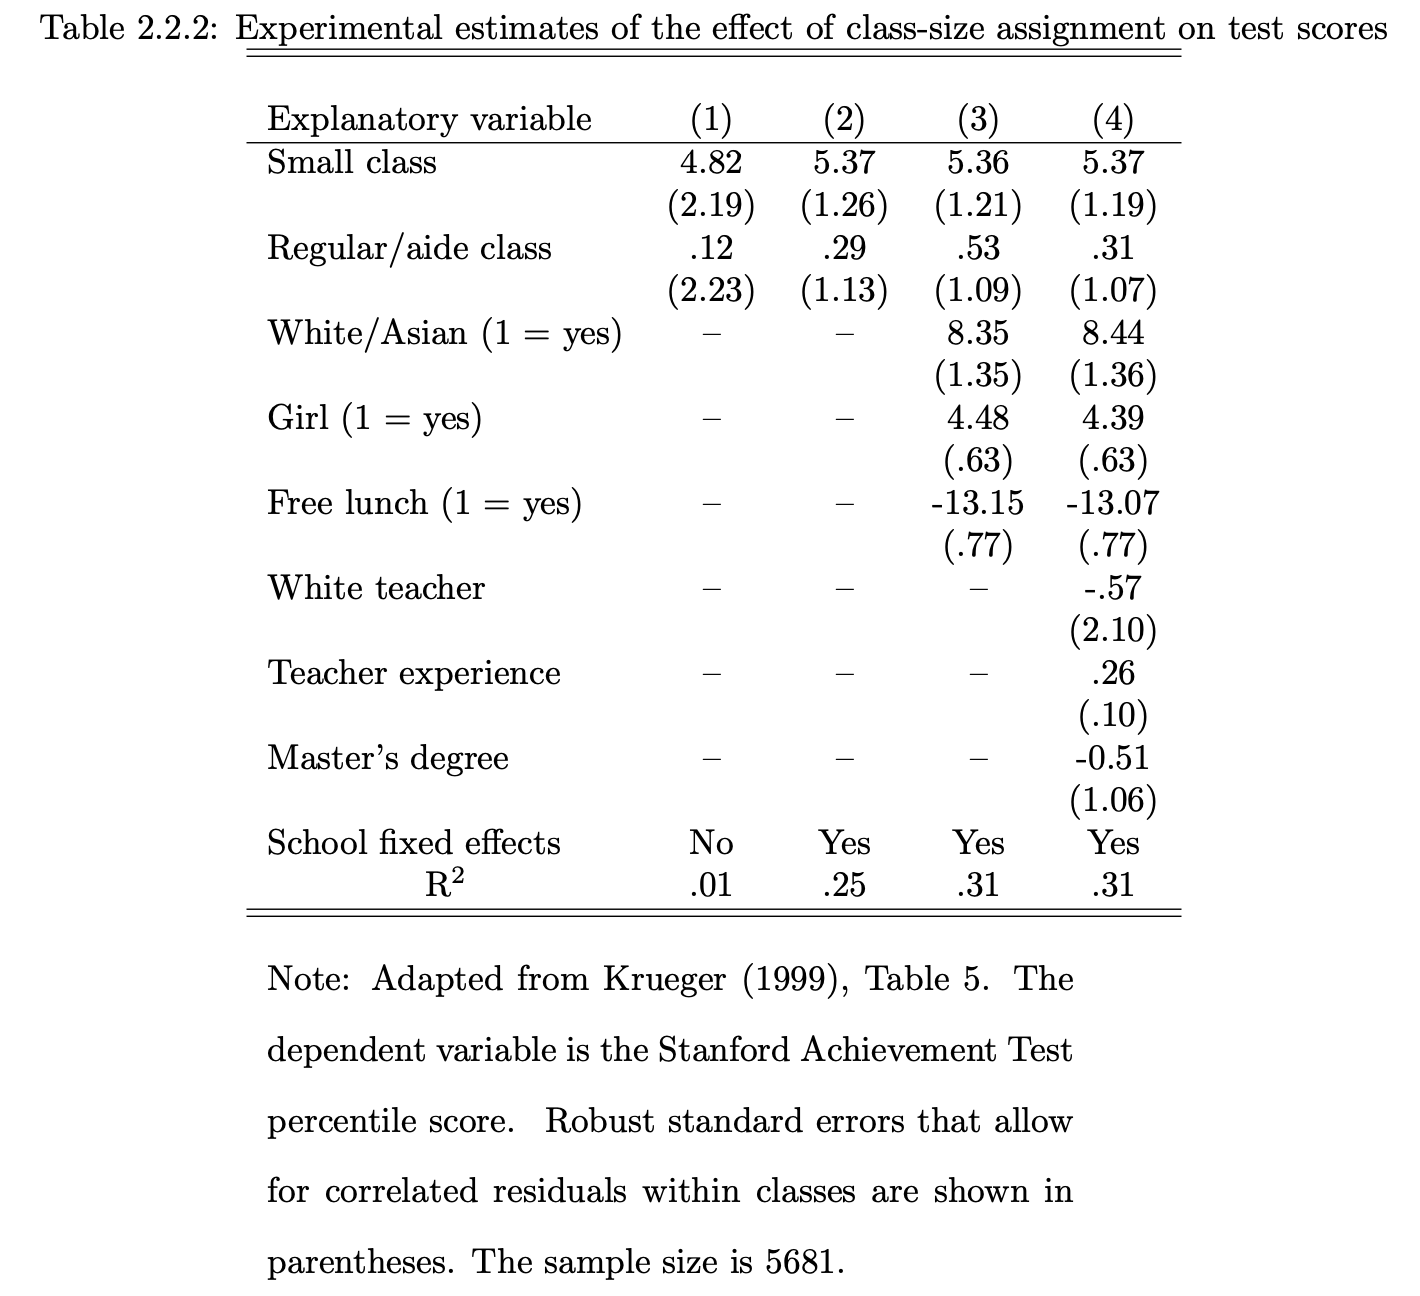
\includegraphics[scale=0.3]{figures/star2.png}
  %\\
  %\tiny
  %Source: motorcycle data from \url{https://www.stata-press.com/data/r12/r.html}
\end{figure}

\end{frame}
%----------------------------------------------------------------------%
\begin{frame}[fragile]
\frametitle{Model Selection When the Goal is Causal Inference}

\begin{itemize}
  \item Traditional approach: researcher selects $X_i$
  \medskip
  \pause 
  \item Problem: mistakes can occur.
  \medskip
  \item Same if they use an ``automatic'' model selection approach. 
  \medskip
  \item Why?
  \pause 
  \item It can leave out potentially important variables with small coefficients but non zero coefficients out
\end{itemize}  

  \end{frame}
%----------------------------------------------------------------------%
\begin{frame}[fragile]
\frametitle{Model Selection When the Goal is Causal Inference}


\begin{itemize}
  \item The omission of such variables then generally contaminates estimation and inference results based on the selected set of variables. (e.g. OVB)
  \medskip
  \item The validity of this approach is delicate because it relies on perfect model selection.
  \medskip
  \item Because model selection mistakes seem inevitable in realistic settings, it is important to develop inference procedures that are robust to such mistakes.
  \medskip
  \item Solution here: Lasso
\end{itemize}


\end{frame}
%----------------------------------------------------------------------%
\begin{frame}[fragile]
\frametitle{Model Selection When the Goal is Causal Inference}
\begin{itemize}
\item Using Lasso is useful for prediction
\medskip
\item However, naively using Lasso  to draw inferences about model parameters can be problematic.
\medskip
\item Part of the difficulty is that these procedures are designed for prediction, not for inference  
\medskip
\item Leeb and Pötscher 2008 show that methods that tend to do a good job at prediction can lead to incorrect conclusions when inference is the main objective
\end{itemize}
\end{frame}


%----------------------------------------------------------------------%
\begin{frame}[fragile]
\frametitle{Model Selection When the Goal is Causal Inference}


\begin{itemize}  
\item Leeb and Pötscher 2008 show that methods that tend to do a good job at prediction can lead to incorrect conclusions when inference is the main 
\medskip
\item This observation suggests that more desirable inference properties may be obtained if one focuses on model selection over the predictive parts of the economic problem
\begin{itemize}
\item The reduced forms and first-stages—rather than using model selection in the structural model directly.
\end{itemize}

\end{itemize}

\end{frame}
%----------------------------------------------------------------------%
\begin{frame}[fragile]
\frametitle{Approximate sparse models}

\begin{itemize}
  \item To fix ideas suppose we have the following model and we want to predict $y$ based on $X$
  \begin{align}
  y_i=g(X_i) + \zeta_i
  \end{align}
  with 
  \begin{itemize}
    \item $E(\zeta_i|g(x_i))=0$
    \item $i=1,\dots,n$ are iid
    \item To avoid over-fitting and produce good out of sample prediction we will need to restrict or regularize $g(.)$
    \item Belloni's et. all approach focuses on an approach that treats $g(X_i)$ as a high-dimensional but that we can approximate linearly
  
  \end{itemize}
\end{itemize}

\end{frame}
%----------------------------------------------------------------------%
\begin{frame}[fragile]
\frametitle{Approximate sparse models}
\begin{align}
    g(X_i)=\sum_{j=1}^p \beta_j x_{ij} +r_{pi}
    \end{align}

\begin{itemize}
    \item where $p>>n$ and $r_{pi}$ is small enough 
    \medskip
    \item Approximate sparsity of this high-dimensional linear model imposes the restriction that linear combinations of only $s<<n$ $x_{ij}$ variables provide a good approximation to $g(X_i)$
    \medskip
    \item A bonus is that the identity of this $s$ $x_{ij}$ variables are a priori unknown
    \medskip
    \item And that we can have a nonzero approximation error $r_{pi}$
    \medskip
    \item We are going to try to learn the identities of these variables while estimating the coefficients.

\end{itemize}

\end{frame}
%----------------------------------------------------------------------%
\begin{frame}[fragile]
\frametitle{Approximate sparse models}
\begin{itemize}

\item We can use Lasso that is slightly modified
\begin{align}
L(\beta) &= \sum_{i=1}^n (y_i-\beta_0 - \sum_{j=1}^p x_{ij}\beta_j)^2 + \lambda \sum_{j=2}^p |\beta_j| \gamma_j
\end{align}

\begin{itemize}
  \item where $\lambda>0$ is the penalty level chosen using  Belloni, Chen, Chernozhukov, and Hansen (2012)
  \medskip
  \item $\gamma_j$ are {\it penalty loadings}
  \medskip
  \item  {\it penalty loadings} are chosen to insure equivariance of coefficient estimates to rescaling of $x_{ij}$ and can also be chosen to address heteroskedasticity, clustering, and non-gaussian errors

\end{itemize}
\end{itemize}

\end{frame}
%----------------------------------------------------------------------%
\begin{frame}[fragile]
\frametitle{Inference with Selection among Many Controls}

\begin{itemize}
  \item Under the approximate sparse models assumption
  \medskip
  \item We consider a linear model where a treatment variable, $D_i$, is taken as exogenous after conditioning on control variables
\begin{align}
y_i = \alpha D_i + X_i'\theta_y +r_{yi} + \zeta_i
\end{align}

\item where $E[\zeta_i|d_i,x_i,r_{yi}]=0$ 
\item $X_i$ is a p-dimensional vector with $p>>n$, but approximately sparse
\item $r_{yi}$ is an approximation error
\item the parameter of interest is $\alpha$

\end{itemize}
\end{frame}
%----------------------------------------------------------------------%
\begin{frame}[fragile]
\frametitle{Inference with Selection among Many Controls}


\begin{itemize}
  \item Naive approach 
  \begin{align}
    y_i = \alpha D_i + X_i'\theta_y +r_{yi} + \zeta_i
  \end{align}
  \begin{itemize}
  \item Select control variables by applying Lasso, forcing the treatment variable to remain in the model
  \medskip
  \item  One could then try to estimate and do inference about $\alpha$ by applying ordinary least squares with $y_i$ as the outcome, and $D_i$ and any selected control variables as regressors. 
  \medskip
  \pause
  \item Are there any problems?
  \end{itemize}
\end{itemize}

\end{frame}
%----------------------------------------------------------------------%
\begin{frame}[fragile]
\frametitle{Inference with Selection among Many Controls}
\begin{itemize}

\item The problem is that it target prediction $\rightarrow$ any variable that is highly correlated to the treatment variable will tend to be dropped 
\medskip
\item  Of course, the exclusion of a variable that is highly correlated to the treatment will lead to substantial omitted-variables bias 
\medskip
\item It ignores a key component to understanding omitted-variables bias, the relationship between the treatment variable and the controls. 
\medskip

\end{itemize}


\end{frame}
%----------------------------------------------------------------------%
\begin{frame}[fragile]
\frametitle{Inference with Selection among Many Controls}
\begin{itemize}
\item The naive approach is based on a “structural” model where the target is to learn the treatment effect given controls, not an equation representing a prediction rule for $y_i$ given $D_i$ and $X_i$. 
\medskip
\item Let's look it this way

\begin{align}
D_i = X_i'\theta_d + r_{di}+v_i
\end{align}

\begin{itemize}
  \item where $E[v_i|X_i,r_{di}]=0$
  \medskip
  \item but some $\theta_d \neq 0$
\end{itemize}
\item The model we are interested is:

\begin{align}
y_i = \alpha D_i + X_i'\theta_y +r_{yi} + \zeta_i
\end{align}
 

\end{itemize}

\end{frame}
%----------------------------------------------------------------------%
\begin{frame}[fragile]
\frametitle{Inference with Selection among Many Controls}
\begin{itemize}

\item It is thus useful to transform $y_i = \alpha D_i + X_i'\theta_y +r_{yi} + \zeta_i$  to a reduced form (recall $D_i = X_i'\theta_d + r_{di}+v_i$):

\begin{align}
y_i &= X_i'(\alpha \theta_d +  \theta_y) + (\alpha r_{di} + r_{yi}) + r_{di}+ (\alpha v_i +\zeta_i) = X_i' \pi + r_{ci} + \epsilon_i \\ \nonumber
\end{align}
\item where $E(\epsilon_i | x_i,r_{ci}]=0$ 
\item $r_{ci}$ is a composite approximation error
\item this equation now represent a predictive relationship, which may be estimated using high-dimensional methods. 


\end{itemize}

\end{frame}


%----------------------------------------------------------------------%
\begin{frame}[fragile]
\frametitle{Inference with Selection among Many Controls}

\begin{itemize}


\item To prevent model selection mistakes, it is important to consider both equations for selection.
\medskip
\item We apply variable selection methods to each of the two reduced form equations and then use all of the selected controls in estimation of $\alpha$. 
\medskip
\item We select
\begin{enumerate}
\item A set of variables that are useful for predicting $y_i$, say $X_{yi}$, and 
\item A set of variables that are useful for predicting $D_i$, say $X_{di}$.

\end{enumerate}
\item We then estimate $\alpha$ by ordinary least squares regression of $y_i$ on $D_i$ and the union of the variables selected for predicting $y_i$ and $D_i$, contained in $X_{yi}$ and $X_{di}$. 



%Using both variable selection steps immunizes the resulting procedure against the types of model selection mistakes discussed above for single-equation procedures. Specififically, using the variables selected in both reduced form equations ensures that any variables that have large effects in either the “structural” equation for yi or the reduced form equation for di are included in the model. Any excluded variables are therefore at most mildly associated to yi and di, which greatly limits the scope for omitted-variables bias. It is also noteworthy that the “double selection” procedure implicitly estimates the residuals εi and vi and then regresses the estimates of εi on the estimates of vi to construct an estimator of α, thereby providing a selection analog of Robinson’s (1988) method for estimating the parameters of a partially linear model to the high-dimensional case.
\end{itemize}



\end{frame}

%----------------------------------------------------------------------%
\begin{frame}[fragile]
\frametitle{Inference with Selection among Many Controls}


   \begin{figure}[H] \centering
            \captionsetup{justification=centering}
              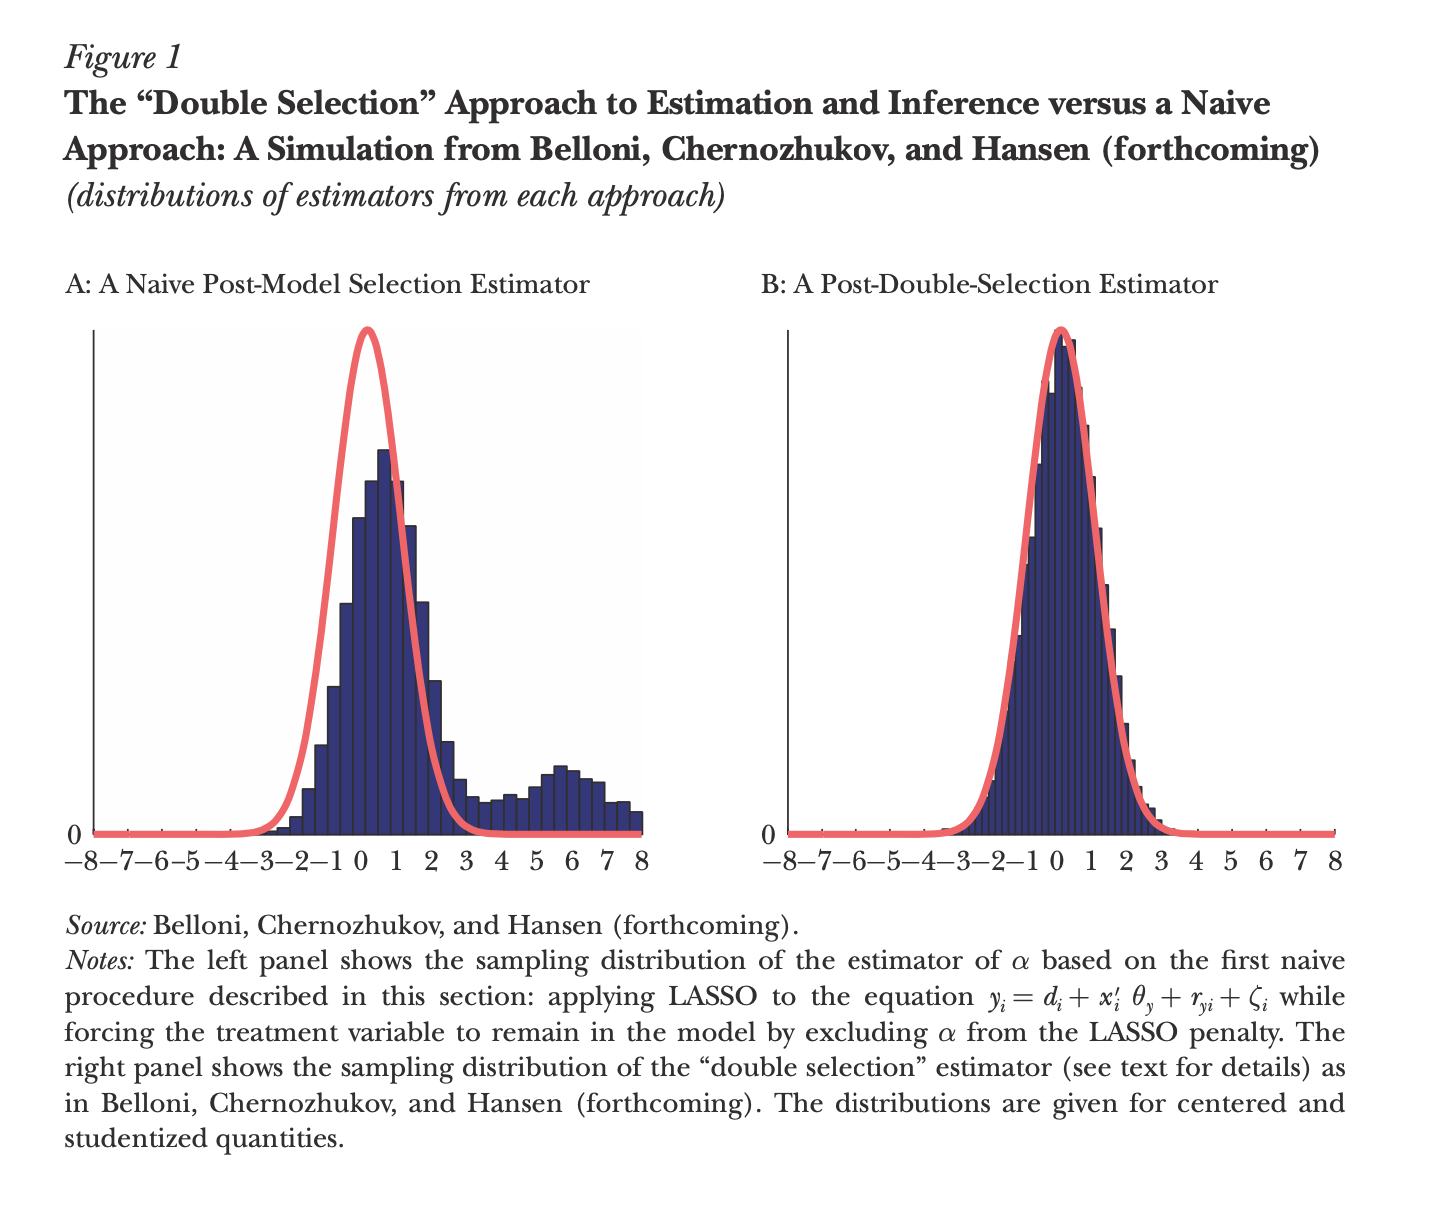
\includegraphics[scale=0.30]{figures/fig1_belloni}
 \end{figure}

\begin{itemize}
\item We are making sure that we use variables that are important for either of the two predictive relationships to guard against OVB
\end{itemize}
\end{frame}
%----------------------------------------------------------------------%
\section{Application}
%----------------------------------------------------------------------%
\begin{frame}[fragile]
\frametitle{Application: Estimation of the treatment effect in a linear model with many confounding factors}

\begin{itemize}
\item What is the effect of an initial (lagged) level of GDP per capita on the growth rates of GDP per capita?
\medskip
\item Solow-Swan-Ramsey growth model predicts convergence
\medskip
\item Poorer countries should typically grow faster and therefore should tend to catch up with the richer countries, conditional on a set of institutional and societal characteristics. 
\medskip
\item Covariates that describe such characteristics include variables measuring education and science policies, strength of market institutions, trade openness, savings rates and others.
\end{itemize}

\end{frame}
%----------------------------------------------------------------------%
\begin{frame}[fragile]
\frametitle{Application: Estimation of the treatment effect in a linear model with many confounding factors}


Thus, we are interested in a specification of the form:

\begin{align}
y_i = \alpha d_i+ \sum_{j=1}^p \beta_j x_{ij} + \varepsilon_i
\end{align}

where
\begin{itemize}
\item  \(y_i\) is the growth rate of GDP over a specified decade in country \(i\), 
\item \(d_i\) is the log of the initial level of GDP at the beginning of the specified period, 
\item \(x_{ij}\)'s form a long list of country \(i\)'s characteristics at the beginning of the specified period. 
\item We are interested in testing the hypothesis of convergence,  \(\alpha < 0\).
\end{itemize}


 

\end{frame}
%----------------------------------------------------------------------%
\begin{frame}[fragile]
\frametitle{Application: Estimation of the treatment effect in a linear model with many confounding factors}
For this exercise we use the Barro and Lee (1994) data


\begin{Shaded}
\begin{Highlighting}[]
\KeywordTok{require}\NormalTok{(}\StringTok{"hdm"}\NormalTok{) }\CommentTok{\#package}
\KeywordTok{data}\NormalTok{(GrowthData) }\CommentTok{\#load data}
\KeywordTok{dim}\NormalTok{(GrowthData)}
\end{Highlighting}
\end{Shaded}

\begin{verbatim}
## [1] 90 63
\end{verbatim}

The number of covariates \(p\) is large relative to the sample size \(n\)

\begin{Shaded}
\begin{Highlighting}[]
\NormalTok{y =}\StringTok{ }\NormalTok{GrowthData[,}\DecValTok{1}\NormalTok{,drop=F]}
\NormalTok{d =}\StringTok{ }\NormalTok{GrowthData[,}\DecValTok{3}\NormalTok{, drop=F]}
\NormalTok{X =}\StringTok{ }\KeywordTok{as.matrix}\NormalTok{(GrowthData)[,}\OperatorTok{{-}}\KeywordTok{c}\NormalTok{(}\DecValTok{1}\NormalTok{,}\DecValTok{2}\NormalTok{,}\DecValTok{3}\NormalTok{)]}
\NormalTok{varnames =}\StringTok{ }\KeywordTok{colnames}\NormalTok{(GrowthData)}
\end{Highlighting}
\end{Shaded}

\end{frame}
%----------------------------------------------------------------------%
\begin{frame}[fragile]
\frametitle{Application: Estimation of the treatment effect in a linear model with many confounding factors}

\begin{itemize}
\item Now we can estimate the effect of the initial GDP level. 
\item First, we estimate by OLS:
\end{itemize}


\begin{Shaded}
\begin{Highlighting}[]
\NormalTok{xnames=}\StringTok{ }\NormalTok{varnames[}\OperatorTok{{-}}\KeywordTok{c}\NormalTok{(}\DecValTok{1}\NormalTok{,}\DecValTok{2}\NormalTok{,}\DecValTok{3}\NormalTok{)] }\CommentTok{\# names of X variables}
\NormalTok{dandxnames=}\StringTok{ }\NormalTok{varnames[}\OperatorTok{{-}}\KeywordTok{c}\NormalTok{(}\DecValTok{1}\NormalTok{,}\DecValTok{2}\NormalTok{)] }\CommentTok{\# names of D and X variables}

\CommentTok{\# create formulas by pasting names (this saves typing times)}
\NormalTok{fmla=}\StringTok{ }\KeywordTok{as.formula}\NormalTok{(}\KeywordTok{paste}\NormalTok{(}\StringTok{"Outcome \textasciitilde{} "}\NormalTok{, }\KeywordTok{paste}\NormalTok{(dandxnames, }\DataTypeTok{collapse=} \StringTok{"+"}\NormalTok{)))}

\CommentTok{\# Estimate using OLS}
\NormalTok{ls.effect=}\StringTok{ }\KeywordTok{lm}\NormalTok{(fmla, }\DataTypeTok{data=}\NormalTok{GrowthData)}
\end{Highlighting}
\end{Shaded}

\end{frame}
%----------------------------------------------------------------------%
\begin{frame}[fragile]
\frametitle{Application: Estimation of the treatment effect in a linear model with many confounding factors}

Second, we estimate the effect by the partialling out by Post-Lasso:

\begin{Shaded}
\begin{Highlighting}[]
\NormalTok{dX =}\StringTok{ }\KeywordTok{as.matrix}\NormalTok{(}\KeywordTok{cbind}\NormalTok{(d,X))}
\NormalTok{lasso.effect =}\StringTok{ }\KeywordTok{rlassoEffect}\NormalTok{(}\DataTypeTok{x=}\NormalTok{X, }\DataTypeTok{y=}\NormalTok{y, }\DataTypeTok{d=}\NormalTok{d, }\DataTypeTok{method=}\StringTok{"partialling out"}\NormalTok{)}
\KeywordTok{summary}\NormalTok{(lasso.effect)}
\end{Highlighting}
\end{Shaded}

\begin{verbatim}
## [1] "Estimates and significance testing of the effect of target variables"
##      Estimate. Std. Error t value Pr(>|t|)    
## [1,]  -0.04981    0.01394  -3.574 0.000351 ***
## ---
## Signif. codes:  0 '***' 0.001 '**' 0.01 '*' 0.05 '.' 0.1 ' ' 1
\end{verbatim}

\end{frame}
%----------------------------------------------------------------------%
\begin{frame}[fragile]
\frametitle{Application: Estimation of the treatment effect in a linear model with many confounding factors}

Third, we estimate the effect by the double selection method:

\begin{Shaded}
\begin{Highlighting}[]
\NormalTok{dX =}\StringTok{ }\KeywordTok{as.matrix}\NormalTok{(}\KeywordTok{cbind}\NormalTok{(d,X))}
\NormalTok{doublesel.effect =}\StringTok{ }\KeywordTok{rlassoEffect}\NormalTok{(}\DataTypeTok{x=}\NormalTok{X, }\DataTypeTok{y=}\NormalTok{y, }\DataTypeTok{d=}\NormalTok{d, }\DataTypeTok{method=}\StringTok{"double selection"}\NormalTok{)}
\KeywordTok{summary}\NormalTok{(doublesel.effect)}
\end{Highlighting}
\end{Shaded}

\begin{verbatim}
## [1] "Estimates and significance testing of the effect of target variables"
##          Estimate. Std. Error t value Pr(>|t|)   
## gdpsh465  -0.05001    0.01579  -3.167  0.00154 **
## ---
## Signif. codes:  0 '***' 0.001 '**' 0.01 '*' 0.05 '.' 0.1 ' ' 1
\end{verbatim}


\end{frame}
%----------------------------------------------------------------------%
\begin{frame}[fragile]
\frametitle{Application: Estimation of the treatment effect in a linear model with many confounding factors}

\begin{itemize}
\item Collecting the results
\end{itemize}
\bigskip
\bigskip

\begin{table}[ht]
\centering
\begin{tabular}{rrr}
  \hline
 & Estimate & Std. Error \\ 
  \hline
full reg via ols & -0.01 & 0.02989 \\ 
  partial reg
via post-lasso  & -0.05 & 0.01394 \\ 
  partial reg via double selection & -0.05 & 0.01579 \\ 
   \hline
\end{tabular}
\end{table}

\end{frame}
%----------------------------------------------------------------------%
\section{Review \& Next Steps}
%----------------------------------------------------------------------%
\begin{frame}
\frametitle{Review \& Next Steps}
  
\begin{itemize} 
    \item Today:
    
    \item Elastic Net
    \medskip
    \item Lasso for Causality: Post Lasso Double Selection


    \bigskip  
  \item  Next class:  Classification


\bigskip  

\end{itemize}
\end{frame}
%----------------------------------------------------------------------%
\section{Further Readings}
%----------------------------------------------------------------------%
\begin{frame}
\frametitle{Further Readings}
\scriptsize
\begin{itemize}

  \item Belloni, A., Chernozhukov, V., \& Hansen, C. (2014). Inference on treatment effects after selection among high-dimensional controls. The Review of Economic Studies, 81(2), 608-650.
  \medskip
  \item Belloni, A., Chernozhukov, V., \& Hansen, C. (2014). High-dimensional methods and inference on structural and treatment effects. Journal of Economic Perspectives, 28(2), 29-50.
  \medskip
  \item Chernozhukov, V.,  Hansen, C., \& Spindler, M (2016). hdm: High-Dimensional Metrics R Journal, 8(2), 185-199.  \url{https://journal.r-project.org/archive/2016/RJ-2016-040/index.html}
  \item Friedman, J., Hastie, T., \& Tibshirani, R. (2001). The elements of statistical learning (Vol. 1, No. 10). New York: Springer series in statistics.
  \medskip
  \item James, G., Witten, D., Hastie, T., \& Tibshirani, R. (2013). An introduction to statistical learning (Vol. 112, p. 18). New York: springer.
  \medskip
  \item Zou, H. \& Hastie, T. (2005). Regularization and variable selection via the elastic net. Journal of the Royal StatisticalSociety, Series B.67: pp. 301–320
\end{itemize}

\end{frame}






%----------------------------------------------------------------------%
%----------------------------------------------------------------------%
\end{document}
%----------------------------------------------------------------------%
%----------------------------------------------------------------------%

